\documentclass[twocolumn]{report}

\usepackage[toc,page]{appendix}
\usepackage{amsmath, amsfonts, amssymb, amsthm}
\usepackage{tikz}
\renewcommand\thesection{\arabic{section}}
\allowdisplaybreaks
\newtheorem{definition}{Definition}
\newtheorem{theorem}{Theorem}
\newtheorem{observation}{Observation}

\newcommand\cone[1]{\textrm{cone}(#1)}
\newcommand\conv[1]{\textrm{conv}(#1)}
\newcommand\R{\mathbb R}
\newcommand\N{\mathbb N}
\newcommand\Z{\mathbb Z}

\title{Optimization Handbook}
\author{Henri Lefebvre}

\begin{document}
    \maketitle
    \tableofcontents

    \part{Linear Optimization}
    \chapter{Introduction}
    \chapter{Lagrangian duality}
    \chapter{The Simplex algorithm}

In chapter \ref{chap:lp}, we showed with the fundamental theorem of linear programming that the search space for optimality was reduced indeed to the set of extreme points of the feasible region, or equivalently of basic feasible solutions for the problem. The idea of the Simplex algorithm is to go from one extreme point to another in such a way that the objective function is always improved (i.e., decreases in case of a minimization). By assumption, the considered polyhedron is lower bounded (upper bounded in case of maximization) and therefore, the algorithm reaches the optimal point. The method can be thought of as a travel from an original extreme point to the one which maximizes the objective function. 

The name Simplex comes from the name of the geometrical generalization of triangles to higher dimensions. Its name comes from the idea that it is the "simplest" closed geometrical object in $n$ dimension. 

The first section derives the algorithm formally. Then we explain in more details the geometrical interpretation of the Simplex algorithm. Since the algorithm starts with an initial basic feasible solution, the next section will explain how such a point can be found by using the same Simplex algorithm. In the three last sections, we give the pseudo code of the Revised Simplex algorithm written in matrix form and introduce two variants of the Simplex : (1) the bounded simplex which deals with bounded variables and (2) the transportation Simplex which is used for transportation problems. 

\section{Formal derivation}

\subsection{Assumptions}

For the sake of demonstrations, we introduce the following assumption : 
\begin{assumption}[Nondegeneracy assumption]
    Every basic feasible solution is a nondegenerate basic
feasible solution.
\end{assumption}

\subsection{Pivoting and Gauss reduction}

In this section, we explain how one can move from one basic solution to another with a standard operation from linear algebra called pivoting. This operation is used in Gauss method for solving a system of linear equations. Consider the following set of equations :
\begin{align*}
&a_{11}x_1 + a_{12}x_2 + ... + a_{1n}x_n = b_1 \\
&a_{21}x_1 + a_{22}x_2 + ... + a_{2n}x_n = b_2 \\
&\vdots \qquad\qquad\qquad\quad\ddots\qquad \vdots \\
&a_{m1}x_1 + a_{m2}x_2 + ... + a_{mn}x_n = b_m
\end{align*}
Of course, it is well known that if $m < n$ and if the equations are not redondant (i.e., they are linearly independent) there is not a unique solution. Yet, following the princple of pivoting from the Gauss elimination technique (see appendix \ref{chap:linear_algebra}) one can turn this system in a so-called \textit{canonical form} expressed as 
\begin{equation*}
    \resizebox{\linewidth}{!}{$
    \begin{array}{ccccccccccccc}
        x_1 & + & \overline a_{1(m+1)}x_{m+1} & + & ... & + & \overline a_{1n}x_n & = & \overline b_1 \\
        x_2 & + & \overline a_{2(m+1)}x_{m+1} & + & ... & + & \overline a_{2n}x_n & = & \overline b_2 \\
        x_3 & + & \overline a_{3(m+1)}x_{m+1} & + & ... & + & \overline a_{3n}x_n & = & \overline b_3 \\
        \vdots & & \vdots & & & \ddots  & & & \vdots\\
        x_m & + & \overline a_{m(m+1)}x_{m+1} & + & ... & + & \overline a_{mn}x_n & = & \overline b_m \\
    \end{array}
    $
    }
\end{equation*}
which we often write, for the sake of synthesis, in a so-called \textit{tableau} :
\begin{equation*}
    \begin{array}{cccccccc|c}
        x_1 & x_2 & x_3 & ... & x_m & x_{m+1} & ... & x_n \\\hline
        1 & 0 & 0 & 0 & 0 & \overline a_{1(m+1)} & ... & \overline a_{1n} & \overline b_1 \\
        0 & 1 & 0 & 0 & 0 & \overline a_{2(m+1)} & ... & \overline a_{2n} & \overline b_2 \\
        0 & 0 & 1 & 0 & 0 & \overline a_{3(m+1)} & ... & \overline a_{3n} & \overline b_3 \\
        & & & \ddots & & \vdots & \ddots & & \vdots\\
        0 & 0 & 0 & 0 & 1 & \overline a_{m(m+1)} & ... & \overline a_{mn} & \overline b_m \\
    \end{array}
\end{equation*} It is clear that if one posesses a system of equations written in cannonical form, then the solution given by $x = (\overline b_1, \overline b_2, ..., \overline b_m, 0, 0, ...., 0)$ is a basic solution. The idea of the Simplex algorithm is, in fact, to pivot from one canonical form to another. The question however is how to select the variable which will enter the basis and which one will leave the basis in order to increase a given objective function. This is deatailed in the following sub-sections. 

\subsection{Vector leaving the basis}

\subsubsection{First approach}

In this section, we show how one can decide which variable should leave the basis. In fact, in the previous section, we showed that the pivot operation allows us to move from a basic solution to another, however, such a move does not guarantee the feasibility of the obtained basic solution. In other words, it is not established that the pivot operation will keep the positivity of the variables. We present here a sufficient condition for the pivot operation to keep the feasibility property when moving from one basic solution to another. 

Let $x$ be a basic solution. We have \[ a_1x_1 + a_2x_2 + ... + a_mx_m = b \] where $x_i>0, \forall i = 1...m$ (nondegeneracy assumption). And suppose that we want to bring $x_q$ in the basis. The question is how to choose which variable has to leave the basis in order to keep feasibility of the new basic solution. For that purpose, let us write $a_q$ in terms of the current basis : \[ a_q = \lambda_1 a_1 + \lambda_2 a_2 + ... + \lambda_m a_m \] From the two above equalities, we derive the following : {\small \[ (x_1 - \varepsilon \lambda_1)a_1 + (x_2 - \varepsilon\lambda_2)a_2 + ... + (x_m - \varepsilon\lambda_m)x_m + \varepsilon a_q = b \]} for any $\varepsilon > 0$, which is a linear combination of at most $m+1$ vectors. Setting $\varepsilon = 0$ yields the current basic feasible solution. As $\varepsilon$ increases, the coefficient of $a_q$ increases. Yet, it yields a non basic variable, in general. The coefficients of the other vectors may increase or decrease with $\varepsilon$ depending on the original coefficients (i.e., if we have $\lambda_i > 0$). Therefore, by taking the first value of $\varepsilon$ which makes vanishing such a vector, we ensure the feasibility of the obtained new basic solution. Formally, we choose $\varepsilon$ such that : 
\[ \varepsilon = \min\{ x_i/\lambda_i : \lambda_i > 0 \} \] If the minimum is achieved by more than one variable, the new basic feasible solution is degenerate. If, however, none of the $\lambda_i$ are positive, this means that all the coefficients increase as $\varepsilon$ increases, without restriction, while keeping feasibility. This corresponds to a case where the polyhedron is unbounded. 

\subsubsection{Alternative approach}

Another approach for reaching the same result is to consider a problem in standard form and to notice that we can always write a basic feasbile solution like so : 
\[ \overline b_i - \sum_{j=m}^{n} \overline a_{ij}x_j \ge 0 \qquad\forall i = 1,...,m \]
We want to increase a non-basic variable $x_q$ while keeping feasibility. Also, we'd like to increase $x_q$ as much as we can. That is, we keep the other non-basic solutions to zero. This yields :
\[ \overline b_i \ge \overline a_{ij}x_q\qquad\forall i=1,...,m \]
Thus, it follows that :
\[
    \begin{cases}
        \dfrac{\overline b_i}{\overline a_{ij}} \ge x_q & \forall i = 1,...,m | \overline a_{ij} > 0\\
        \dfrac{\overline b_i}{\overline a_{ij}} \le x_q & \forall i = 1,...,m | \overline a_{ij} < 0\\
    \end{cases}
\]
Note that when $\overline a_{ij} < 0$, no upper bound on $x_q$ can be derived. Hence, when all the $a_{ij}$ coefficients are negative, the problem is unbounded. On the contrary, when at least one coeeficient is negative, we do have a constraint on $x_q$ and to ensure feasibility with respect to all the constraints, one should increase $x_q$ by \[ \min\left\{ \frac{\overline b_j}{\overline a_{ij}} : \overline a_{ij} > 0 \right\} \] which implies setting $x_k$ to zero where $k$ denotes the argmin of the above finite minimum. We get is the same result as in the first approach. 

\subsection{Vector entering the basis}

In the previous section, we have shown how to choose which variable had to leave in order to keep feasibility when we want to insert a given variable in the basis. In that sense, it allows us to travel from one basic solution to another while keeping feasibility. In this section, we show how to choose which variable should enter the basis in order to increase a given objective function. For that purpose, consider the following objective function : \[ c^Tx = c_1x_1 + c_2x_2 + ... + c_nx_n \] And consider a feasible basic solution $\hat x = [\hat x_B, 0]$. Its objective value is given by \[ c_1\hat x_1 + c_2\hat x_2 + ... + c_m\hat x_m \] If we write our system of equalities in canonical form, recall that we trivially have $x_j = \overline b_j$ for basic variables and $x_j = 0$ for non-basic variables. The key idea here, is to express the objective function value of a general solution $x$ in terms of the objective value of the basic solution $\hat x$. First note that the following holds for any feasible solution $x$ :
\begin{align*}
    x_1 &= \overline b_1 - \sum_{j=m+1}^p \overline a_{1j}x_j \\
    x_2 &= \overline b_2 - \sum_{j=m+1}^p \overline a_{2j}x_j \\
    \vdots & \qquad\qquad \vdots \\
    x_m &= \overline b_m - \sum_{j=m+1}^p \overline a_{mj}x_j \\
\end{align*} By substituting the basic variables from $\hat x$ by the above equalities, we get :
\begin{align*}
    &c^Tx = \sum_{j=1}^n c_jx_j\\
    &= \sum_{j=1}^m c_jx_j + \sum_{j=m+1}^n c_jx_j\\
    &= \sum_{j=1}^m c_j\left( \overline b_j - \sum_{k=m+1}^n \overline a_{jk}x_k \right) + \sum_{j=m+1}^n c_jx_j\\
    &= \sum_{j=1}^m c_j\overline b_j - \sum_{j=1}^m \sum_{k=m+1}^n c_j\overline a_{jk}x_k + \sum_{j=m+1}^n c_jx_j\\
    &= \sum_{j=1}^m c_j\overline b_j - \sum_{k=m+1}^nx_k\left(\sum_{j=1}^m c_j\overline a_{jk}\right) + \sum_{j=m+1}^n c_jx_j\\
    &= \sum_{j=1}^m c_j\hat{x}_j + \sum_{j=m+1}^n x_j\left( c_j - \sum_{i=1}^m \overline a_{ij}c_i \right)\\
    &= c^T_B\hat x_B + \sum_{j=m+1}^n (c_j - z_j)x_j
\end{align*}
where \[ z_j = \sum_{i=1}^m \overline a_{ij}c_i \] This result gives us a condition for a vector to benificially enter the basis. Indeed, if, for a given variable $j$, we have $c_j - z_j < 0$ then it means that increasing the value of $x_j$ from zero to a positive value will decrease the objective function. Hence, going from the solution $\hat x$ to another solution which includes $x_j > 0$ will yield a lower value of the objective. 

We introduce the standard notation $r_j = c_j - z_j$. These coefficients are called \textit{reduced cost} or \textit{relative costs} since they measure the cost of a variable respectively to a given basis. We can interpret these numbers as the gain we would obtain to use a real variable $x_j$ instead of the linear combination giving $x_j = \sum_{j=1}^m \overline a_j x_j $. Another interpretation is to see the reduced cost as the amount by which the objective cost would have to decrease (for minimization problems) in order to make the entrance of a column profitable. 

We now can state the two following theorems : 
\begin{theorem}
    Given a non-degenerate basic feasible solution with corresponding objective value $z_0$. If there exist a column such that $c_j - z_j < 0$, then there is a feasible solution with objective value $z < z_0$. If the column $\overline a_j$ can be substituted for some vector in the original basis to yield a feasible basic solution, then this solution will have an objective value $z < z_0$. If, however, $\overline a_j$ cannot be substituted to yield a basic feasible solution, the problem is unbounded and the optimal solution tends to minus infinity. 
\end{theorem}
\begin{theorem}[Optimality condition]
    If, for some basic feasible solution, $c_j - z_j\ge 0$ for all $j$, then the solution is optimal. 
\end{theorem}

\section{Finding a feasible solution}

As previously explained the Simplex procedure needs an initial feasible point to start. A practical way to obtain one is by solving an optimization problem whose solution is an extreme point of the feasible region and for which we do know a feasible solution. This step is called the Phase I of the Simplex. The idea is to introduce \textit{artificial} variables which are not part of the original problem and to replace the original objective by the minimization of a positive sum of the artifical variables. Clearly, since we do not constrain the artifical variables, a feasible solution for that problem is to select all the artifical variables and to set the rest to zero. Its objective value is simply the number of added artifical variables. Solving this problem, if a feasible solution exists, the Simplex will find one since it would not contain any artifical variable and its cost would therefore be minimal. 

Formally, to find a feasible solution for the feasible region  $\{ x\in\R^n_+ | Ax = b \}$, one has to solve the folowing problem 
\begin{align*}
    \textrm{minimize } & \sum_{k=1}^m x_{n+k}\\
    \textrm{s.t. } & Ax = b\\
    & x_j \ge 0\quad\forall j=1...n+m
\end{align*}
For which an initial feasible solution is clearly given by $(\underbrace{0,\quad...,\quad0}_{n\textrm{ original variables}},\underbrace{1,\quad...,\quad1}_{m\textrm{ artifical variables}})$. 

\section{The Simplex method}

\subsection{Pseudo-code}

The Simplex method takes as input a feasible basic solution. We assume that we start the algorithm with a canonical form of $Ax = b$. We append a row at the bottom of this tableau, obtained the so-called \textit{Simplex Tableau}, in which we report the reduced costs and the objective function in the corner. The Simplex Tableau is presented in table \ref{tab:simplex}. 
\begin{table}[h!]
    \centering
    \begin{tabular}{ccccccc|cc}
        $x_1$ & $x_2$ & $...$ & $x_m$ & $x_{m+1}$ & $...$ & $x_n$ & $b$ \\\hline
        1 & 0 & $...$ & 0 & $\overline a_{1(m+1)}$ & $...$ & $\overline a_{1n}$ & $\overline b_1$\\
        0 & 1 & $...$ & 0 & $\overline a_{2(m+1)}$ & $...$ & $\overline a_{2n}$ & $\overline b_2$\\
        $\vdots$ &  & $\ddots$ & $\vdots$ & $\vdots$ & $\ddots$ & $\vdots$ & $\vdots$  \\
        0 & 0 & $...$ & 1 & $\overline a_{m(m+1)}$ & $...$ & $\overline a_{mn}$ & $\overline b_m$\\\hline
        0 & 0 & $...$ & 0 & $r_{m+1}$ & $...$ & $r_n$ & $-z_0$
    \end{tabular}
    \caption{The Simplex Tableau}
    \label{tab:simplex}
\end{table}

Regarding the last row of the tableau, we may interpret it as $z$ being an extra variable subject to the constraint $z = \sum_{j=1}^n c_jx_j$. A basic solution would therefore be of size $m+1$, yet we can require that $z$ must be part of it. For that reason, it is not necessary to add a column in the tableau for $z$ since it would always be equal to $(0,0,...,0,1)$. Therefore, initially, the last row contains the objective cost of each variables and a right hand side of zero. By pivoting in order to put the system into standard form, the last row's values for basic variables can also be reduced to zero. This is, in fact, equivalent to transforming $c^Tx = z$ into \[ r_{m+1}x_{m+1} + r_{m+2}x_{m+2} + ... + r_nx_n - z = -z_0 \] Where $r_j$ denotes the reduced cost of variable $x_j$. The Simplex algorithm is stated in \ref{alg:simplex}. 

\begin{algorithm}[h!]
    \caption{Simplex Algorithm}
    \label{alg:simplex}
    \begin{description}
        \item[Step 0] : From a system in canonical form, compute the reduced costs by row reduction on the last row
        \item[Step 1] : If each $r_j \ge 0$, STOP. The solution is optimal.
        \item[Step 2] : Find $q$ such that $r_q < 0$ to determine which variable will enter the basis.
        \item[Step 3] : Find the variable with corresponding minimum ratio $\min\{ \overline b_i/\overline a_{iq} : \overline a_{iq} > 0 \}$. Let $p$ be the index of that variable.\\
        If there is no coefficient $\overline a_{iq} > 0$, STOP. The problem is unbounded, the solution in $-\infty$.
        \item[Step 4] : Pivot every rows (including the last one) on the $pq$th element. Go to \textbf{Step 1}.
    \end{description}
\end{algorithm}


\section{Degeneracy}

Running the Simplex algorithm, it is possible to find degenerate basic feasible solutions. In most cases, these degenerate solutions can be handled in the same way as any basic feasible variable. Yet, in some situations, it is that, having a current degenerate feasible basic solution, one computes the variable to enter the basis and the associated minimum ratio to be zero. In this case, a zero valued basic variable will enter the basis while not improving the objective function. In this case, it may occur that the Simplex enters in an infinite cycle, going from one degenerate solution to another degenerate solution. 

This section is devoted to the study of such cases. First, we give an example of Simplex cycling, then, give some pivot rules to avoid cycling.

\subsection{Example}

The example we give here was introduced in \cite{gollinear}. 
TODO

\subsection{Pivot Rules}
\subsubsection{Dantzig's Rule}
\subsubsection{Bland's Rule}
\subsubsection{Steepest-edge rule}
\subsubsection{Approximate steepest-edge rule}
\subsubsection{Partial pricing}

TODO

\subsection{Examples}
\subsubsection{Optimal solution}

Le us consider the following problem :
\begin{align*}
    \textrm{maximize } & x_1 + x_2\\
    \textrm{s.t. } & 4x_1 + x_2 \le 20\\
    & x_1 + 2x_2 \le 11\\
    & x_1, x_2\ge 0
\end{align*}
The first step to do is to write this problem in standard form by introducing two slack variables $s_1$ and $s_2$ and to turn this maximization problem into a minimization problem like so :
\begin{align*}
    \textrm{minimize } & -x_1 - x_2\\
    \textrm{s.t. } & 4x_1 + x_2 + s_1 = 20\\
    & x_1 + 2x_2 + s_2 = 11\\
    & x_1, x_2, s_1, s_2\ge 0
\end{align*}
This gives us a good Simplex Tableau to start with. Indeed, the slack variables already form a basis to start with and setting $s_1 = 20$ and $s_2 = 11$ is a basic feasible solution. The initial tableau is :
\begin{center}
    \begin{tabular}{cccc|c}
        $x_1$ & $x_2$ & $s_1$ & $s_2$ & $b$ \\\hline
        4 & 1 & 1 & 0 & 20\\
        1 & 2 & 0 & 1 & 11\\\hline
        -1 & -1 & 0 & 0 & 0
    \end{tabular}
\end{center}
Where we see that variables $x_1$ and $x_2$ are elligeable to enter the basis (i.e., have negative reduced costs). We'll use the "most negative reduced cost" rule for pivoting, i.e., the variable which leaves the basis corresponds to the one having the most negative reduced cost. In our case, both negative-reduced-cost variables have a reduced cost of $-1$. We arbitraly use $x_2$. Then, we compute the ratios for positive values of the column $\overline b_i / \overline a_{i2}$. The minimum one is $\min(20/1 ; 11/2) = 5.5$ and is reached in the second row. Thus, $s_2$ exits the basis. After pivoting on $2,2$, the resulting tableau is :
\begin{center}
    \begin{tabular}{cccc|c}
        $x_1$ & $x_2$ & $s_1$ & $s_2$ & $b$ \\\hline
        $\frac 72$ & 0 & 1 & $-\frac 12$ & $\frac{29}2$\\
        $\frac 12$ & 1 & 0 & $\frac 12$ & $\frac{11}2$\\\hline
        $-\frac 12$ & 0 & 0 & $\frac 12$ & $\frac{11}2$
    \end{tabular}
\end{center}
Here, only variable $x_1$ has a negative reduced cost. Thus, $x_1$ will enter the basis. Naturally, $s_1$ will leave the basis since $\min(\frac{29}{2}/\frac{7}2 ; \frac{11}2/\frac 12) = \frac{29}7$. This leads to the following table :
\begin{center}
    \begin{tabular}{cccc|c}
        $x_1$ & $x_2$ & $s_1$ & $s_2$ & $b$ \\\hline
        1 & 0 & $\frac 27$ & $-\frac 17$ & $\frac{29}7$\\
        0 & 1 & $-\frac 17$ & $\frac 47$ & $\frac{24}7$\\\hline
        0 & 0 & $\frac 17$ & $\frac 37$ & $\frac{53}7$
    \end{tabular}
\end{center}
Here, every non basic reduced cost are positive, the Simplex algorithm terminates and the solution is optimal. Figure \ref{fig:simplex_step} depicts the travel made by the Simplex algorithm throughout its execution. The initial basic solution is $(0,0)$, then goes to $(0,11/2)$ and finally reaches the optimal solution $(29/7,24/7)$.

\begin{figure}[h!]
    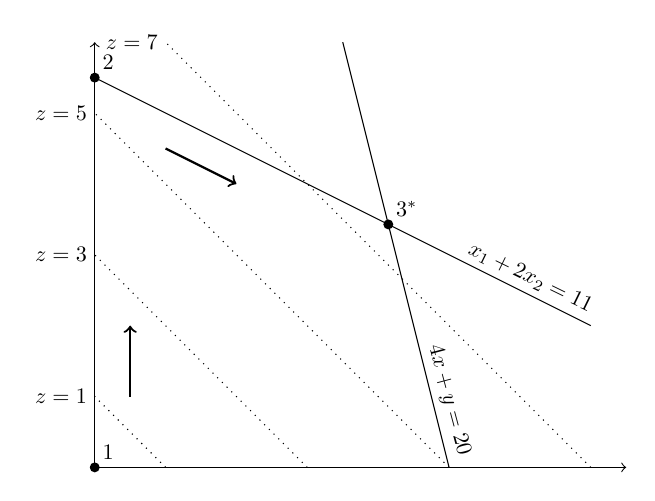
\begin{tikzpicture}[scale = .9]
        \draw[<->] (0,6) |- (7.5,0);
        \draw (3.5,6) -- (5,0) node[above left, rotate=-75, scale = .8] {$4x+y = 20$};
        \draw (7,2) node[scale = .8, rotate=-26, above left] {$x_1+2x_2=11$} -- (0,5.5);
        \fill (0,0) circle (2pt) node[above right, scale = .8] {1};
        \fill (0,5.5) circle (2pt) node[above right, scale = .8] {2};
        \fill (29/7,24/7) circle (2pt) node[above right, scale = .8] {$3^*$};
        \draw[thick] (.5, 1) edge[->] (.5, 2);
        \draw[thick] (1, 4.5) edge[->] (2, 4);

        \draw[dotted] (1,0) -- (0,1) node[left, scale=.8] {$z = 1$};
        \draw[dotted] (3,0) -- (0,3) node[left, scale=.8] {$z = 3$};
        \draw[dotted] (5,0) -- (0,5) node[left, scale=.8] {$z = 5$};
        \draw[dotted] (7,0) -- (1,6) node[left, scale=.8] {$z = 7$};
    \end{tikzpicture}
    \caption{Example of Simplex moves}
    \label{fig:simplex_step}
\end{figure}

\subsubsection{Unbounded problem}

In this section, we consider the optimization problem stated below. It is our intention that the problem is unbounded, i.e., its optimal solution goes to infinity. The goal of this example is to show how the Simplex algorithm terminates in such situations and what are the informations which are still usable in such cases. Consider the following :
\begin{align*}
    \textrm{maximize } & 2x_1 + x_2\\
    \textrm{s.t. } & 2x_1 - x_2 \ge -5\\
    & x_1 - x_2 \le 2\\
    & x_1, x_2\ge 0
\end{align*}
Clearly, the feasible region is unbounded as it can be seen in figure \ref{fig:unbounded_simplex}. Note that the Simplex works even with unbounded polyhedron and is able to compute optimal solution in such cases. The specificty of this problem is that the plane defining the objective function is "oriented" (i.e., is increasing) towards the unbounded direction. In chapter \ref{chap:benders}, we give a sufficient condition for a problem to be bounded implying the extreme rays of a polyhedron. In this case, the objective function and the extreme rays of the feasible region are oriented in the same direction. 

\begin{figure}[h!]
    \centering
    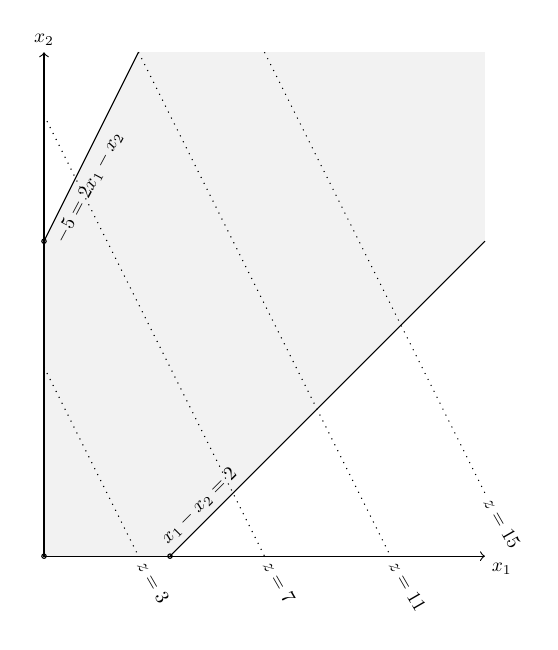
\begin{tikzpicture}[scale=.8, every node/.style={scale = .7}]
        \fill[gray!10] (1.5, 8) -- (0,5) -- (0,0) -- (2,0) -- (7,5) -- (7,8);
        \draw (0,5) circle (1pt) node[below right, rotate = 62] {$-5 = 2x_1 - x_2$} -- (1.5, 8);
        \draw (0,0) circle (1pt);
        \draw (2,0) circle (1pt) node[above right, rotate = 45] {$x_1 - x_2 = 2$} -- (7,5);
        \draw[<->] (0,8) node[above] {$x_2$} |- (7,0) node[below right] {$x_1$};
        \draw[dotted] (0,3) -- (1.5,0) node[right, rotate = -60] {$z = 3$};
        \draw[dotted] (0,7) -- (3.5,0) node[right, rotate = -60] {$z = 7$};
        \draw[dotted] (1.5,8) -- (5.5,0) node[right, rotate = -60] {$z = 11$};
        \draw[dotted] (3.5,8) -- (7,1) node[right, rotate = -60] {$z = 15$};
    \end{tikzpicture}
    \caption{Unbounded feasible region}
    \label{fig:unbounded_simplex}
\end{figure}

First, let us write the considered problem in standard form by introducing the slack variables and turning the maximization problem into a minimization problem, this gives :
\begin{align*}
    \textrm{minimize } & -2x_1 - x_2\\
    \textrm{s.t. } & -2x_1 + x_2 + s_1 = 5\\
    & x_1 - x_2 + s_2 = 2\\
    & x_1, x_2, s_1, s_2\ge 0
\end{align*}
We introduce the Simplex tableau of this problem : 
\begin{center}
    \begin{tabular}{cccc|c}
        $x_1$ & $x_2$ & $s_1$ & $s_2$ & $b$ \\\hline
        -2 & 1 & 1 & 0 & 5\\
        1 & -1 & 0 & 1 & 2\\\hline
        -2 & -1 & 0 & 0 & 0
    \end{tabular}
\end{center} Looking at the most negative reduced cost, we determine that $x_1$ will enter the basis and by, computing the minimum ratios, that $s_2$ will leave the basis. We get : \begin{center}
    \begin{tabular}{cccc|c}
        $x_1$ & $x_2$ & $s_1$ & $s_2$ & $b$ \\\hline
        0 & -1 & 1 & 2 & 9\\
        1 & -1 & 0 & 1 & 2\\\hline
        0 & -3 & 0 & 2 & 2
    \end{tabular}
\end{center} Again, looking at the most negative reduced cost, we can see that $x_2$ should enter the basis. However, there are no positive coefficient in that row. This means that we can increase $x_2$ as much as we want while keeping feasibility (i.e., there are no feasibility restrictions). Thus, we conclude that the problem is unbounded. Yet, how can we interpret the vector $(-1, -1)^T$ returned by the Simplex ? Answer : it is the opposite direction an the extreme ray of the feasible region. 
\[ d = \begin{pmatrix} 1\\ 1 \end{pmatrix} \]

\subsubsection{Reduced costs}
\paragraph{Computation}
In this section, we suppose having a canonical tableau of the problem from the first example : 
\begin{center}
    \begin{tabular}{cccc|c}
        $x_1$ & $x_2$ & $s_1$ & $s_2$ & $b$ \\\hline
        $\frac 72$ & 0 & 1 & $-\frac 12$ & $\frac{29}2$\\
        $\frac 12$ & 1 & 0 & $\frac 12$ & $\frac{11}2$\\
        % $-\frac 12$ & 0 & 0 & $\frac 12$ & $\frac{11}2$
    \end{tabular}
\end{center} where the reduced costs are missing. We show by example how to compute the reduced costs. 

First, note that $(s_1, x_2)$ is a basis of $\R^2$ ($m = 2$). Thus, the associated reduced costs are $0$. Concerning the non-basic variables, we can compute the reduced costs using the formula $r_j = c_j - z_j$ where $z_j = \sum_{i=1}^m \overline a_{ij}c_i$. We recall here the objective function : $c^Tx = -x_1 - x_2$. Therefore, we have :
{\small \begin{align*}
    r_{x_1} &= -1 - \sum_{i=1}^m \overline a_{i1}c_i = -1 - \left( \frac 72\times 0 + \frac 12 \times -1 \right)\\
    &= -\frac 12\\
    r_{s_2} &= 0 - \sum_{i=1}^m \overline a_{i1}c_i = 0 - \left( -\frac 12\times 0 + \frac 12 \times -1 \right)\\
    &= \frac 12
\end{align*}}
Finally, we easily compute the objective value :  {\small \[ z = c^Tx = -1 \times 0 + (-1) \times \frac{11}2 + 0 \times \frac{29}2 + 0\times 0 = -\frac{11}{2} \]}

\paragraph{Interpreation}
In this short example, we show the interpretation of the reduced costs as the increase in the variable's objective cost necessary to make the entrance of the variable in the basis profitable. Indeed, consider the (very dumb) following problem :
\begin{align*}
    \textrm{maximize } & 4x_1 + x_2\\
    \textrm{s.t. } & x_1 + x_2 \le 1\\
    & x_1, x_2\ge 0
\end{align*}

First, let us write this problem in standard form by turning the maximization into a minimization problem and by introducing slack variables :
\begin{align*}
    \textrm{minimize } & -4x_1 - x_2\\
    \textrm{s.t. } & x_1 + x_2 + s = 1\\
    & x_1, x_2, s\ge 0
\end{align*} The feasible region of the problem is depicted in figure \ref{fig:feasible_reduced} in the top plot as well as the levels of the objective function. We can easily see that the optimal solution (marked by a $*$ in the plot) is $(1,0)$. Let us run the Simplex algorithm for that problem :
\begin{center}
    \begin{tabular}{ccc|c}
        $x_1$ & $x_2$ & $s$ \\\hline
        1 & 1 & 1 & 1\\\hline
        -4 & -1 & 0 & 0
    \end{tabular}
    $\rightarrow$
    \begin{tabular}{ccc|c}
        $x_1$ & $x_2$ & $s$ \\\hline
        1 & 1 & 1 & 1\\\hline
        0 & 3 & 4 & 4
    \end{tabular}
\end{center}
First, we look for the most negative reduced cost. This indicates that $x_1$ will enter the basis. Since we are in one dimension, the basis is composed of a single element. Therefore, the leaving variable is simply the variable forming the current basis, i.e., $s$. In two steps, the Simplex terminates and we can see that the reduced cost of variable $x_2$ is $r_2 = 3$. This means that, if we increase the cost $c_2$ of at least $x_2$ in the objective function, it may be profitable to include $x_2$ in the basis. Indeed, in the second plot from figure \ref{fig:feasible_reduced}, we depicted the objective function with an increase in $c_2$ of exactely $r_2$. We can see that the objective function reaches its maximum value simultaneously in $(0,1)$ and in $(1,0)$. In the last plot however, we increased even more the cost $c_2$ for variable $x_2$ while keeping the other costs constant. We can see that now, the optimal solution is realised in $(0,1)$.

\begin{figure}[h!]
    \centering
    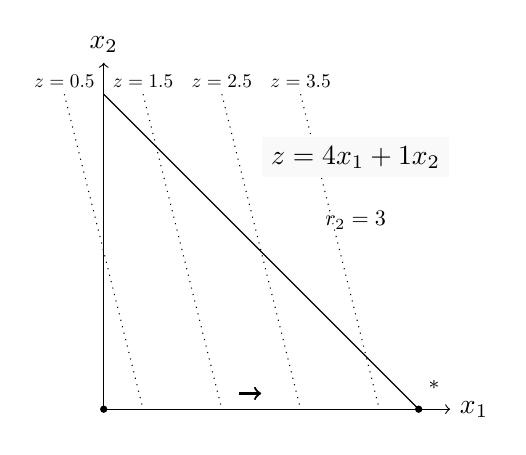
\begin{tikzpicture}[scale = 4]
        \draw[<->] (0,1.1) node[above] {$x_2$} |- (1.1, 0) node[right] {$x_1$};
        \draw (0,1) -- (1,0);
        \fill[black] (0,0) circle (.33pt);
        \fill[black] (1,0) circle (.33pt) node[above right] {$\vphantom{z}^*$};
        \draw (.43,.05) edge[thick, ->] (.5,.05);
        \foreach \l in {0.5, 1.5, 2.5, 3.5}
            \draw[dotted] ( \l/4 - 1/4, 1 ) node[above, scale = .7] {$z = \l$} -- (\l/4,0);
        \draw (.8,.8) node[fill=gray!5] {$z=4x_1 + 1x_2$};
        \draw (.8, .6) node[scale=.8] {$r_2 = 3$};
    \end{tikzpicture}
    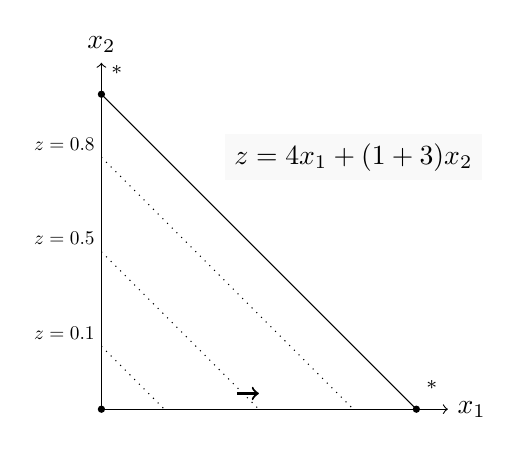
\begin{tikzpicture}[scale = 4]
        \draw[<->] (0,1.1) node[above] {$x_2$} |- (1.1, 0) node[right] {$x_1$};
        \draw (0,1) -- (1,0);
        \fill[black] (0,0) circle (.33pt);
        \fill[black] (1,0) circle (.33pt) node[above right] {$\vphantom{z}^*$};
        \fill[black] (0,1) circle (.33pt) node[above right] {$\vphantom{z}^*$};
        \draw (.43,.05) edge[thick, ->] (.5,.05);

        \draw[dotted] (0,.8) node[above left, scale = .7] {$z = 0.8$} -- (.8,0);
        \draw[dotted] (0,.5) node[above left, scale = .7] {$z = 0.5$} -- (.5,0);
        \draw[dotted] (0,.2) node[above left, scale = .7] {$z = 0.1$} -- (.2,0);
        \draw (.8,.8) node[fill=gray!5] {$z=4x_1 + (1+3)x_2$};
    \end{tikzpicture}
    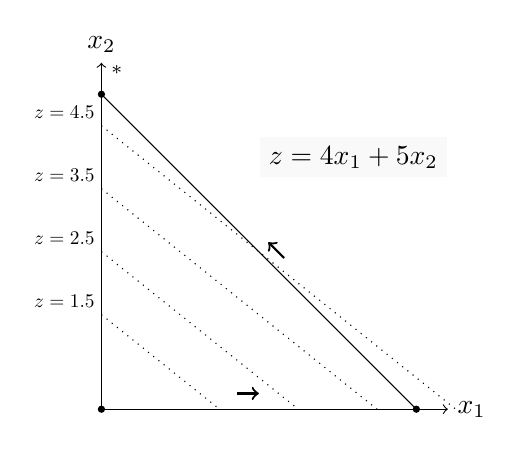
\begin{tikzpicture}[scale = 4]
        \draw[<->] (0,1.1) node[above] {$x_2$} |- (1.1, 0) node[right] {$x_1$};
        \draw (0,1) -- (1,0);
        \fill[black] (0,0) circle (.33pt);
        \fill[black] (1,0) circle (.33pt);
        \fill[black] (0,1) circle (.33pt) node[above right] {$\vphantom{z}^*$};
        \draw (.43,.05) edge[thick, ->] (.5,.05);
        \draw (.53,.53) edge[thick, <-] (.58,.48);

        \draw[dotted] (0,.9) node[above left, scale = .7] {$z = 4.5$} -- (1.125,0);
        \draw[dotted] (0,.7) node[above left, scale = .7] {$z = 3.5$} -- (.875,0);
        \draw[dotted] (0,.5) node[above left, scale = .7] {$z = 2.5$} -- (.625,0);
        \draw[dotted] (0,.3) node[above left, scale = .7] {$z = 1.5$} -- (.375,0);
        \draw (.8,.8) node[fill=gray!5] {$z=4x_1 + 5x_2$};
    \end{tikzpicture}
    \caption{Interpretation of the reduced cost}
    \label{fig:feasible_reduced}
\end{figure}

    \chapter{Relaxation techniques}

\section{Formal definition}

\section{Linear relaxation}

\section{Lagrangian relaxation}

\section{Surrogate relaxation}
    \chapter{The branch-and-bound algorithm}
    \chapter{The branch-and-cut algorithm}
    \chapter{Column generation and the branch-and-price algorithm}
    \chapter{Benders decomposition}
\label{chap:benders}

\section{Introduction}

Benders decomposition is a solution method for solving certain large-scale optimization problems. It is particularly suited for problems in which a set of variables are said to be \textit{complicating} in the sense that fixing them to a given value makes the problem easy. Briefly, the Benders decomposition approach seperates an original problem into several decision stages. A first-stage \textit{master} problem is solved using only a subset of variables, then, the values of the remaining variables are determined by a so-called \textit{subproblem} depending on the first-stage variables. If the master problem's optimal solution yields an infeasible subproblem, a \textit{feasibility cut} is added to the master problem, which is then re-solved. Due to the structure of the reformulation, the Benders algorithm starts with a \textit{restricted master problem} where only a subset of constraints are considered while the others are iteratively added. 

This technique was first introduced in \cite{Benders1962} and has since been generalized to non-linear mixed integer problems. 

\section{Formal derivation}

Consider the following problem :
\begin{align}
    \textrm{minimize } & c^Tx + f(y) \\
    \textrm{s.t. } & Ax + g(y) = b \\
    & y\in Y, x\ge 0
\end{align} where variable $y$ is a \textit{complicating constraint}. Note that it may be complicating due to the form of $f$ or $g$ but also by our ability to enforce the constraint $y\in Y$. We assume that fixing $y$ to a given value $\hat y$ turns our problem into an easy-to-solve problem. 

We can notice that our problem is equivalent to the following one : \[
    \min\left\{ f(y) + \min\left\{ c^Tx : Ax = b - g(y) \right\} : y \in Y \right\}
\] Let us denote by $q(y)$ the value of the minimization problem over $x$ : $q(y) = \min\{ c^Tx : Ax = b - g(y) \}$. By duality, the following holds \[
    q(y) = \max\{ (b-g(y))^T\pi : A^T\pi \le c \}
\] Note that the feasibility space of the dual does not depend on the values of $y$ and let us apply the decomposition theorem for polyhedra \ref{th:decomposition_polyhedra} on it :
\begin{align*}
    &\{ A^T\pi \le c \} = \left\{ \sum_i u^i\alpha_i + \sum_j v^j\beta_j \right\} \\
    &\sum_i \alpha_i = 1 \quad\textrm{and}\quad \alpha, \beta \ge 0
\end{align*} where $\{u^i\}_i$ denotes the extreme points of $\{x|Ax\le c\}$ and $\{v^j\}_j$ denotes the extreme rays of the polyhedral cone $\{x|Ax\le 0\}$. Intuitively, the convex combination of the extreme points of $\{x|Ax\le c\}$ defines the optimal solutions (since we know that there exists at least one optimal solution corresponding to an extreme point of the considered polyhedron) while the conical combination of extreme rays of $\{x|Ax\le 0\}$ defines the feasibility region. The following theorem will allow us to reformulate our problem :
\begin{theorem}
    \label{th:upper_bounded_problem_theorem}
    Let ($\mathcal P$) be the following problem : \[ \max\{ c^Tx : Ax \le b, x\ge 0 \} \tag{$\mathcal P$} \] Then, ($\mathcal P$) is upper bounded if and only if 
    \[ c^Tv^j \le 0\quad \forall j=1,...,J \]
    where $\{v^j\}_{j=1,...,J}$ denotes the set of extreme rays of $\{x|Ax\le 0\}$. 
\end{theorem}
\begin{proof}
$\Rightarrow$ : By contradiction, let us suppose that $(\mathcal P)$ is upper bounded and that there exists $k$ such that $c^Tv^k > 0$. Let us consider a feasible solution to ($\mathcal P$) denoted by $u = z + t$ where $z$ is a convex combination of the extreme points of $\{x|Ax\le b\}$ and $t$ an element of the conical combinations of the extreme rays of $\{x|Ax\le 0\}$ (see theorem \ref{th:decomposition_polyhedra}). Let $\lambda\in\R_+$. Since $v^k$ is in the conical polyhedra $\{x|Ax\le 0\}$, it holds that $\lambda Av^k\le 0$. Moreover, we have $At\le 0$. Hence, $A(t+\lambda v^k)\le 0$. Now, since $v^k\ge 0$, we have $\lambda v^k\ge 0$ and since $t\ge 0$ it holds that $t+\lambda v^k\ge 0$. This shows that, for any $\lambda$, $z+\lambda v^k$ is a feasible solution for problem ($\mathcal P$). However, its associated objective value is given by $c^Tu + \lambda c^Tv^k\rightarrow +\infty$ when $\lambda\rightarrow+\infty$ since, by assumption, $c^Tv^k> 0$. This contradicts the fact that ($\mathcal P$) is upper bounded. \\
$\Leftarrow$ : Let us consider a solution $u = z + t$ then $c^Tu = c^Tz + \sum_j c^Tv^j\beta_j \le c^Tz$ since $c^Tv^j\le 0, \forall j=1,...,J$. Problem ($\mathcal P$) is therefore upper bounded by $\sum_i \alpha_i \max_i\{ c^Tu^i \}$. 
\end{proof}
Theorem \ref{th:upper_bounded_problem_theorem} can be intuitively understood by interpreting $c^Tv^j$ as $\langle c, v^j\rangle$ (scalar product). The necessary and sufficiant condition that $\langle c, v^j\rangle\le 0$ simply expresses that the the hyperplane defining the objective function must be \textit{oriented} (i.e., increasing) in the direction of the origin of the cone formed by the extreme rays of the polyhedron. It is depicted in figure \ref{fig:upper_bounded_problem}.

\begin{figure}[h!]
    \centering
    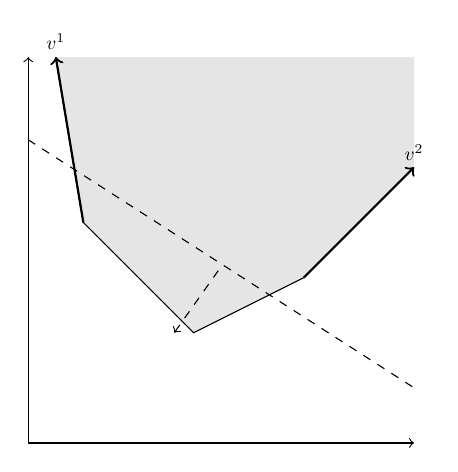
\begin{tikzpicture}[scale=.7, every node/.style = {scale = .7}]
        \draw[<->] (7, 0) -| (0, 7);
        \fill[fill=gray!20] (.5,7) -- (1,4) -- (2,3) -- (3,2) -- (5,3) -- (7,5) -- (7,7) -- cycle;
        \draw (.5,7) -- (1,4) -- (2,3) -- (3,2) -- (5,3) -- (7,5);
        \draw[->, thick] (1,4) -- (.5,7) node[above] {$v^1$};
        \draw[->, thick] (5,3) -- (7,5) node[above] {$v^2$};

        % \draw[dashed] (7,3) node[below] {$c^Tx^1$} -- (3,7);
        % \draw[dashed] (7,1) node[below] {$c^Tx^2$} -- (1,7);
        \draw[dashed] (0,5.5) -- (7, 1) ;%node[below] {$c^Tx^3$};
        % \draw[dashed] (0,4) -- (4, 0) node[below] {$c^Tx^4$};
        \draw[dashed,<-] (2.65,2) -- (3.5,3.2);

        % \draw (3.5, -1.3) node {$c^Tx^4 \ge c^Tx^3\ge c^Tx^2 \ge c^Tx^1$};
    \end{tikzpicture}
    \caption{Illustration of theorem \ref{th:upper_bounded_problem_theorem}}
    \label{fig:upper_bounded_problem}
\end{figure}

If we apply theorem \ref{th:upper_bounded_problem_theorem} to our specific problem, we find that a necessary and sufficient condition for $q(y)$ to be upper bounded is that $(b-g(y))^Tv^j\le 0, \forall j=1,...,J$ where $v^j$ denotes an extreme ray of the polyhedron $\{x|Ax\le c\}$ and $J$ a list for their indices. Moreover, we know that there exists at least one optimal solution realised in an extreme point of the feasible region. Therefore, by calling $u^i, i=1,...,I$ the extreme points of the feasible region, the problem of finding the value of $q(y)$ can be reformulated as \[ q(y) = \min\{ q : q \ge (b-g(y))^Tu^i\quad\forall i=1,...,I \} \] Assuming that this problem is bounded. We finally can write our original problem as the following
\begin{align}
    \textrm{minimize } & f(y) + q\\
    \textrm{s.t. } & y\in Y\\
    & (b-g(y))^Tu^i \le q\quad\forall i=1,...,I \label{eq:optimality_cut}\\
    & (b-g(y))^Tv^j \le 0\quad\forall j=1,...,J \label{eq:feasibility_cut}
\end{align} where constraints \ref{eq:optimality_cut} are called \textit{optimality cuts/constraints} since they define the extreme points of the feasible region and constraints \ref{eq:feasibility_cut} are called \textit{feasibility cuts/constraints} since they enforce that the problem is bounded. 

\section{Algorithm}

\subsection{Pseudo code}

It is clear that our final formulation implies an exponential number of constraints since polyhedra typically have an exponential number of extreme points and extreme rays. The idea of the Benders Decomposition Algorithm is to work with a relaxation of the problem where only a limited number of constraints are considered. The algorithm then tries to reach the optimality of the original problem by a \textit{clever} choice of constraints to be added iteratively. The algorithm is presented in \ref{alg:benders}. 
\begin{algorithm}[h!]
    \caption{Benders Decomposition Algorithm}
    \label{alg:benders}
    \begin{description}
        \item[Step 0] : Find an extreme point of $\{x|Ax\le c, x\ge 0\}$ (e.g., via the phase 1 of the Simplex)\\$1\rightarrow p, 0\rightarrow k$
        \item[Step 1] : Solve relaxed problem with only $p$ optimality constraints and $k$ feasibility constraints :
        \begin{align*}
            \textrm{minimize } & f(y) + q\\
            \textrm{s.t. } & y\in Y\\
            & (b-g(y))^Tu^i \le q\quad\forall i=1,...,p\\
            & (b-g(y))^Tv^j \le 0\quad\forall j=1,...,k
        \end{align*}
        Let $\bar y, \bar q$ be the optimal solution thus obtained. 
        \item[Step 2] : Check the feasible of $(\bar y, \bar q)$ for the original problem by solving \[ q(\bar y) = \max\{ (b-g(y))^T\pi : A^T\pi \le c, \pi\ge 0 \} \]
        Then,
        \begin{description}
            \item[If] $q(\bar y) = +\infty$ : \\
            The problem is unbounded and, from theorem \ref{th:upper_bounded_problem_theorem}, one can find an extreme ray $v^j$ such that $(b-g(y))^Tv^j > 0$. \\
            Add feasibility cut to the relaxed problem.\\
            Increment $k$. \\
            Got to \textbf{Step 1}.
            \item[Else] : \\
            Let $\bar\pi$ be the optimal solution of cost $q(\bar y)$. 
            \begin{description}
                \item[If] $\bar q < q(\bar y)$ :\\
                Add optimality cut $(b-g(y))^T\bar\pi\le q$\\
                Increment $p$.\\
                Got to \textbf{Step 1}.
                \item[Else] :\\
                The solution is optimal.
            \end{description}
        \end{description}
    \end{description}
\end{algorithm}

\subsection{Generating a feasibility cut}

In \textbf{Step 2} of algorithm \ref{alg:benders}, it is asked to find an extreme ray such that $(b-g(y))^Tv^j > 0$, i.e., a direction in which the problem is unbouned. A way to do that is to use the Simplex Tableau. Indeed, if a problem is unbounded, this implies that there exists a variable whose reduced cost is positive (i.e., ready to enter the basis) while the associated column is composed of postive terms (i.e., no constraint bounds its value). The associated column is in fact an extreme ray of the polyhedron. 

\section{Stabilisation methods}

\subsection{Bundle methods}

\subsection{Proximal methods}

\section{Generalization}

In this section, we take interest in a generalization of the Benders decomposition applicable for the following problem
\begin{align}
    \textrm{minimize } & f(x,y) \\
    \textrm{s.t. } & g(x,y) \le 0\\
    & x\in X\\
    & y\in Y
\end{align} under the following hypothesis :
\begin{enumerate}[label=($\roman*$)]
    \item $X$ is a convex set
    \item $f(x,y)$ and $g(x,y)$ are convex-in-$x$ over $X$
\end{enumerate}

Again, we can write the \textit{projection} on the $y$-variable space, thus obtaining : 
\[
    \min\left\{ \inf\{ f(x,y) : g(x,y)\le 0, x\in X \} : y \in Y \right\}
\] and let us denote by $h(y)$ the minimization problem over $x$, i.e., 
\[
    h(y) = \inf\{ f(x,y) : g(x,y)\le 0, x\in X \}
\]
    \chapter{Dantzig-Wolfe decomposition}

    \part{Non-linear Optimization}

    \begin{appendices}
        \chapter{Convexity}

\begin{definition}[Minkowski sum]
    Let $A$ and $B$ be two vector spaces, the Minkowki sum is defined as
    \[
        A + B = \{ a + b | a\in A, b\in B \}
    \]
\end{definition}

\begin{definition}[Convex combination]
    Let $x_1,...,x_n$ be a finite set of vectors in a real vector space, a convex combination of these vectors is a vector of the form 
    \[
        \sum_{i=1}^n\alpha_ix_i\qquad\textrm{with } \sum_{i=1}^k\alpha_i = 1, \alpha\ge 0
    \]
\end{definition}

\begin{definition}[Convex hull]
    \[
        \conv{X} = \left\{ \sum_{i=1}^n\alpha_ix_i \middle| x_i\in X, \sum_{i=1}^n\alpha_i = 1, \alpha\ge 0 \right\}
    \]
\end{definition}

\begin{definition}[Conical combination]
    Let $x_1,...,x_n$ be a finite set of vectors in a real vector space, a conical combination of these vectors is a vector of the form 
    \[
        \sum_{i=1}^k \alpha_ix_i \qquad\textrm{with } \alpha\ge 0
    \]
\end{definition}

\begin{definition}[Conical hull]
\[
    \cone{X} = \left\{ \sum_{i=1}^n \alpha_ix_i \middle| x_i\in X, \alpha_i \ge 0 \right \}
\]
\end{definition}

\begin{theorem}[Affine Minkowski-Weyl]
    Let there be a polytope defined by a set of inequalities, $P = \{ x\in\R^n | Ax\le b \}$. There exists vectors $x_1,...,x_q\in\R^,n$ and $y_1,...,y_r\in\R^n$ such that
    \[
        P = \cone{x_1,...,x_q} + \conv{y_1,...,y_r}
    \]
\end{theorem}

\begin{observation}
    In the affine Minkowki-Weyl theorem, the smallest set of vectors $x_1,...,x_q$ is the set of extreme rays of $P$ and the smallest set of vectors $y_1,...,y_r$ is the set of extreme points of $P$. 
\end{observation}
    \end{appendices}

    \bibliographystyle{abbrv}
    \bibliography{references} 
\end{document}